\documentclass[notes=show]{beamer}
\usepackage{amsmath,amsfonts}
\usetheme{Madrid}
\usecolortheme{seagull}
\setbeamertemplate{navigation symbols}{}

\begin{document}

\title{GMM, Indirect Inference and Bootstrap}
\subtitle{Maximum Likelihood}
\author[Willi Mutschler]{Willi Mutschler}
\date{Winter 2015/2016}
\institute{TU Dortmund}
\maketitle

\section{Maximum likelihood}
\begin{frame}
\begin{itemize}
  \item Make structure of Gradient and score more clear. Analytical example!
  \item Provide tips for optimization!
\end{itemize}
\end{frame}

\begin{frame}\frametitle{Maximum likelihood}\framesubtitle{Basic idea}
\begin{itemize}
    \item The basic idea is very natural:
    \item Choose the parameters such that the probability (likelihood) of the observations $x_{1},\ldots ,x_{n}$ as a function of the unknown parameters $\theta _{1},\ldots ,\theta _{r}$ is maximized
    \item \textbf{Likelihood function}
    \begin{equation*}
        L(\theta ;x_{1},\dots ,x_{n})=\left\{
    \begin{array}{l}
        P(X_{1}=x_{1},\ldots ,X_{n}=x_{n};\theta ) \\[3mm]
        f_{X_{1},\dots ,X_{n}}(x_{1},\dots ,x_{n};\theta )%
    \end{array}
    \right.
    \end{equation*}
\end{itemize}
\end{frame}


\begin{frame}\frametitle{Maximum likelihood}\framesubtitle{Basic idea}
\begin{itemize}
    \item For simple random samples
    \begin{equation*}
        L(\theta ;x_{1},\dots ,x_{n})=\prod_{i=1}^{n}f_{X}(x_{i};\theta )
    \end{equation*}
    \item Maximize the likelihood
    \begin{equation*}
    L(\hat{\theta};x_{1},\ldots ,x_{n})=\max\limits_{\theta \in \Theta }L(\theta;x_{1},\ldots ,x_{n})
    \end{equation*}
    \item ML estimate $\hat{\theta}=\arg \max L(\theta ;x_{1},\ldots ,x_{n})$
    \item ML estimator $\hat{\theta}=\arg \max L(\theta ;X_{1},\ldots ,X_{n})$
\end{itemize}
\end{frame}


\begin{frame}\frametitle{Maximum likelihood}\framesubtitle{Basic idea}
\begin{itemize}
    \item Because sums are easier to deal with than products, \newline
    and because sums are subject to limit laws, it is \newline
    common to maximize the \textbf{log-likelihood}
    \begin{equation*}
        \ln L(\theta )=\sum_{i=1}^{n}\ln f_{X}(X_{i};\theta )
    \end{equation*}
    \item The ML estimator is the same as before, since
    \begin{eqnarray*}
        \hat{\theta} &=&\arg \max \ln L(\theta ;X_{1},\ldots ,X_{n}) \\
        &=&\arg \max L(\theta ;X_{1},\ldots ,X_{n})
    \end{eqnarray*}
    \item Further numerical issues: densities are very small! Solution: it is advisable to multiply it with a factor, ML estimator is unchanged.
\end{itemize}
\end{frame}


\begin{frame}\frametitle{Maximum likelihood}\framesubtitle{Basic idea}
\begin{itemize}
    \item Usually, we find $\hat{\theta}$ by solving the system of equations
    \begin{eqnarray*}
        \partial \ln L/\partial \theta _{1} &=&0 \\
        &\vdots & \\
        \partial \ln L/\partial \theta _{r} &=&0
    \end{eqnarray*}
    \item The gradient vector $g(\theta )=\partial \ln L(\theta )/\partial \theta $ is called \newline
    \textbf{score} \textbf{vector} or score
    \item If the log-likelihood is not differentiable other maximization methods must be used
\end{itemize}
\end{frame}


\begin{frame}\frametitle{Maximum likelihood}\framesubtitle{Example}
\begin{itemize}
    \item Let $X\sim Exp(\lambda )$ with density $f\left( x;\lambda \right) =\lambda e^{-\lambda x}$ for $x\geq 0$ \newline
     and $f\left( x;\lambda \right) =0$ else
    \item Likelihood of i.i.d. random sample
    \begin{equation*}
        L(\lambda ;x_{1},\ldots ,x_{n})=\prod_{i=1}^{n}\lambda e^{-\lambda x_{i}}
    \end{equation*}
    \item Log-likelihood
    \begin{equation*}
        \ln L(\lambda ;x_{1},\ldots ,x_{n})=n\ln \lambda -\lambda \sum_{i=1}^{n}x_{i}
    \end{equation*}
\end{itemize}
\end{frame}


\begin{frame}\frametitle{Maximum likelihood}\framesubtitle{Example}
\begin{itemize}
    \item Set the derivative to zero
    \begin{equation*}
        \frac{\partial \ln L(\lambda )}{\partial \lambda }=\frac{n}{\hat{\lambda}}-\sum\limits_{i=1}^{n}x_{i}\overset{!}{=}0,
    \end{equation*}
    hence
    \begin{equation*}
        \hat{\lambda}=\frac{n}{\sum_{i=1}^{n}x_{i}}=\frac{1}{\bar{x}}
    \end{equation*}
    \item The ML estimator for $\lambda $ is
    \begin{equation*}
        \hat{\lambda}=\frac{1}{\bar{X}}
    \end{equation*}
    consistent but biased!
\end{itemize}
\end{frame}


\begin{frame}\frametitle{Maximum likelihood}\framesubtitle{Properties of ML estimators: Preliminaries}
\begin{itemize}
    \item The log-likelihood and the score vector are
    \begin{eqnarray*}
        \ln L\left( \theta \right) &=&\sum_{i=1}^{n}\ln f_{X}(X_{i};\theta ) \\
        \frac{\partial \ln L\left( \theta \right) }{\partial \theta } &=&\sum_{i=1}^{n}\frac{\partial \ln f_{X}(X_{i};\theta )}{\partial \theta }
    \end{eqnarray*}
    \item The contributions $\ln f_{X}(X_{i};\theta )$ are random variables
    \item The contributions $\partial \ln f_{X}(X_{i};\theta )/\partial \theta $ are random vectors
    \item Hence, limit laws can be applied to the (normalized) sums
\end{itemize}
\end{frame}


\begin{frame}\frametitle{Maximum likelihood}\framesubtitle{Properties of ML estimators: Preliminaries}
\begin{itemize}
    \item For all $\theta $
    \begin{eqnarray*}
        \int e^{\ln L\left( \theta \right) }dx &=&\int L\left( \theta ;x_{1},\ldots,x_{n}\right) dx \\
        &=&1
    \end{eqnarray*}
    since $L\left( \theta \right) $ is a joint density function of $X_{1},\ldots,X_{n}$
\end{itemize}
\end{frame}


\begin{frame}\frametitle{Maximum likelihood}\framesubtitle{Properties of ML estimators: Preliminaries}
\begin{itemize}
    \item Define the matrix $G\left( \theta ,X_{1},\ldots ,X_{n}\right) $ of gradient contributions
    \begin{equation*}
        G_{ij}\left( \theta ,X_{i}\right) =\frac{\partial \ln f_{X}(X_{i};\theta )}{\partial \theta _{j}}
    \end{equation*}
    \item The column sums are the gradient vector with elements
    \begin{equation*}
        g_{j}\left( \theta \right) =\sum_{i=1}^{n}G_{ij}\left( \theta ,X_{i}\right)
    \end{equation*}
    \item The expected gradient vector is $E_{\theta }\left( g\left( \theta \right) \right) =0$\hfill \lbrack P]
\end{itemize}
\end{frame}


\begin{frame}\frametitle{Maximum likelihood}\framesubtitle{Properties of ML estimators: Preliminaries}
\begin{itemize}
    \item The covariance matrix of gradient vector%
    \begin{equation*}
        Cov\left( g\left( \theta \right) \right) =E\left( g\left( \theta \right) g\left( \theta \right) ^{\prime }\right)
    \end{equation*}
    is called information matrix (and often denoted $\mathcal{I}(\theta )$)
    \item Information matrix equality\hfill \lbrack P]
    \begin{eqnarray*}
    Cov\left( g\left( \theta \right) \right) &=&-E\left( H\left( \theta \right)\right) \\
    Cov\left( \frac{\partial \ln L\left( \theta \right) }{\partial \theta }\right) &=&-E\left( \frac{\partial ^{2}\ln L\left( \theta \right) }{\partial\theta \partial \theta ^{\prime }}\right)
    \end{eqnarray*}
\end{itemize}
\end{frame}


\begin{frame}\frametitle{Maximum likelihood}\framesubtitle{Properties of ML estimators}
\begin{enumerate}
    \item Equivariance: If $\hat{\theta}$ is the ML estimator for $\theta $, then $h(\hat{\theta})$ is the ML estimator for $h(\theta )$
    \item Consistency:
    \begin{equation*}
        \textsl{plim}\hat{\theta}_{n}\mathbf{=}\theta
    \end{equation*}
    \item Asymptotic normality:
    \begin{equation*}
        \sqrt{n}\left( \hat{\theta}_{n}-\theta \right) \overset{d}{\rightarrow }  U\sim N\left( 0,V\left( \theta \right) \right)
    \end{equation*}
    \item Asymptotic efficiency: $V\left( {\theta }\right) $ is the Cram\'{e}r-Rao bound
    \item Computability (analytical or numerical); the covariance matrix of the estimator is a by-product of the numerical method
\end{enumerate}
\end{frame}


\begin{frame}\frametitle{Maximum likelihood}\framesubtitle{Properties of ML estimators}
Equivariance:
\begin{itemize}
    \item Let $\hat{\theta}$ be the ML estimator of $\theta $
    \item Let $\psi =h\left( \theta \right) $ be a one-to-one function of $\theta $ with inverse $h^{-1}\left( \psi \right) =\theta $
    \item Then the ML estimator of $\psi $ satisfies
    \begin{equation*}
        \frac{d\ln L\left( h^{-1}\left( \psi \right) \right) }{d\psi }=\frac{d\ln L\left( \theta \right) }{d\theta }\frac{dh^{-1}\left( \psi \right) }{d\psi } =0
    \end{equation*}
    which holds at $\hat{\psi}=h\left( \hat{\theta}\right) $
\end{itemize}
\end{frame}


\begin{frame}\frametitle{Maximum likelihood}\framesubtitle{Properties of ML estimators}
Consistency
\begin{itemize}
    \item The parameter $\theta $ is \textbf{identified} if for all $\theta^{\prime }\neq \theta $ and data $x_{1},\ldots ,x_{n}$
    \begin{equation*}
        \ln L\left( \theta ^{\prime }|x_{1},\ldots ,x_{n}\right) \neq \ln L\left(\theta |x_{1},\ldots ,x_{n}\right)
    \end{equation*}
    \item The parameter $\theta $ is \textbf{asymptotically identified} if for all $\theta ^{\prime }\neq \theta _{0}$
    \begin{equation*}
    \textsl{plim}\frac{1}{n}\ln L\left( \theta ^{\prime }\right) \neq \textsl{plim}\frac{1}{n}\ln L\left( \theta _{0}\right)
    \end{equation*}
    where $\theta _{0}$ is the true value of the parameter\hfill \lbrack P]
\end{itemize}
\end{frame}


\begin{frame}\frametitle{Maximum likelihood}\framesubtitle{Properties of ML estimators}
Asymptotic normality
\begin{itemize}
    \item By definition, the ML estimator satisfies
    \begin{equation*}
        g(\hat{\theta})=0
    \end{equation*}
    \item A first order Taylor series expansion of $g$ around the true parameter vector $\theta _{0}$ gives\hfill \lbrack P]
    \begin{equation*}
        g(\hat{\theta})=g\left( \theta _{0}\right) +H\left( \theta _{0}\right) (\hat{\theta}-\theta _{0})+rest
    \end{equation*}
\end{itemize}
\end{frame}


\begin{frame}\frametitle{Maximum likelihood}\framesubtitle{Covariance matrix estimation}
\begin{itemize}
    \item The (approximate) covariance matrix of $\hat{\theta}$ is
    \begin{equation*}
        Cov(\hat{\theta})=-\left[ E\left( H\left( \theta _{0}\right) \right) \right]^{-1}=-\left[ E\left( \frac{\partial ^{2}\ln L(\theta _{0})}{\partial \theta_{0}\partial \theta _{0}^{\prime }}\right) \right] ^{-1}
    \end{equation*}
    \item A consistent estimator of $Cov(\hat{\theta})$ is
    \begin{equation*}
        \widehat{Cov}(\hat{\theta})=-\left[ H(\hat{\theta})\right] ^{-1}=-\left(\frac{\partial ^{2}\ln L(\hat{\theta})}{\partial \hat{\theta}\partial \hat{\theta}^{\prime }}\right) ^{-1}
    \end{equation*}
    \item Often, $H(\hat{\theta})$ is a by-product of numerical optimization
\end{itemize}
\end{frame}


\begin{frame}\frametitle{Maximum likelihood}\framesubtitle{Covariance matrix estimation}
\begin{itemize}
    \item An alternative consistent covariance matrix estimator is
    \begin{equation*}
        \widehat{Cov}(\hat{\theta})=\left[ G(\hat{\theta};X_{1},\ldots,X_{n})^{\prime }G(\hat{\theta};X_{1},\ldots ,X_{n})\right] ^{-1}
    \end{equation*}
    \item This estimator is called outer-product-of-the-gradient (OPG) estimator
    \item Advantage: Only the first derivatives are required
    \item Disadvantage: Less reliable in small samples
\end{itemize}
\end{frame}


\begin{frame}\frametitle{Maximum likelihood}\framesubtitle{Example}
\begin{itemize}
    \item Numerical estimation of the parameters of $N(\mu ,\sigma ^{2})$
    \item Let $X_{1},\ldots ,X_{50}$ be a random sample from $X\sim N(\mu,\sigma ^{2})$ \newline
    with $\mu =5$ and $\sigma ^{2}=9$
    \item Density function
    \begin{equation*}
        f_{X}(x)=\frac{1}{\sqrt{2\pi }}\exp \left( -\frac{1}{2}\cdot \frac{\left(x-\mu \right) ^{2}}{\sigma ^{2}}\right)
    \end{equation*}
    \item Log-likelihood function $\ln L\left( \mu ,\sigma ^{2}\right)=\sum_{i=1}^{n}\ln f_{X}(x_{i})$
\end{itemize}
\end{frame}


\begin{frame}\frametitle{Maximum likelihood}\framesubtitle{Example}
\begin{itemize}
    \item See \texttt{numnormal.R}
    \item Point estimates
    \begin{equation*}
        \left(
        \begin{array}{c}
        \hat{\mu} \\
        \hat{\sigma}^{2}
        \end{array}
        \right) =\left(
        \begin{array}{c}
        3.64025 \\
        6.90869%
        \end{array}
        \right)
    \end{equation*}
    \item Estimated covariance matrix derived numerically from $H(\hat{\theta})$
    \begin{equation*}
        \widehat{Cov}\left( \hat{\mu},\hat{\sigma}^{2}\right) =\left(
        \begin{array}{rr}
        0.13817 & -0.00016 \\
        -0.00016 & 1.90918
        \end{array}
    \right)
    \end{equation*}
\end{itemize}
\end{frame}


\begin{frame}\frametitle{Maximum likelihood}\framesubtitle{Example}
\begin{itemize}
    \item See \texttt{numnormal.R}
    \item Point estimates
    \begin{equation*}
        \left(
        \begin{array}{c}
        \hat{\mu} \\
        \hat{\sigma}^{2}
        \end{array}
        \right) =\left(
        \begin{array}{c}
        3.64025 \\
        6.90869%
        \end{array}
        \right)
    \end{equation*}
    \item Estimated covariance matrix derived from theory%
    \begin{equation*}
        \widehat{Cov}\left( \hat{\mu},\hat{\sigma}^{2}\right) =\left(
        \begin{array}{cc}
        0.13817 & 0 \\
        0 & 1.90920
        \end{array}
        \right)
    \end{equation*}
\end{itemize}
\end{frame}


\begin{frame}\frametitle{Maximum likelihood}\framesubtitle{Example of violated regularity conditions}
\begin{itemize}
    \item Let $X$ be uniformly distributed on the interval $[0,\theta ]$
    \item The density function is
    \begin{equation*}
        f_{X}\left( x\right) =\left\{
        \begin{array}{ll}
        1/\theta & \quad \text{for }0\leq x\leq \theta \\
        0 & \quad \text{else}
        \end{array}%
        \right.
    \end{equation*}
    \item The likelihood function is
    \begin{equation*}
        L(\theta |x_{1},\ldots ,x_{n})=\left\{
        \begin{array}{ll}
        \left( \frac{1}{\theta }\right) ^{n} & \text{\quad for }\theta \geq
        \max_{i}x_{i} \\[3mm]
        0 & \quad \text{else}
        \end{array}%
        \right.
    \end{equation*}
\end{itemize}
\end{frame}


\begin{frame}\frametitle{Maximum likelihood}\framesubtitle{Example of violated regularity conditions}
\begin{center}
    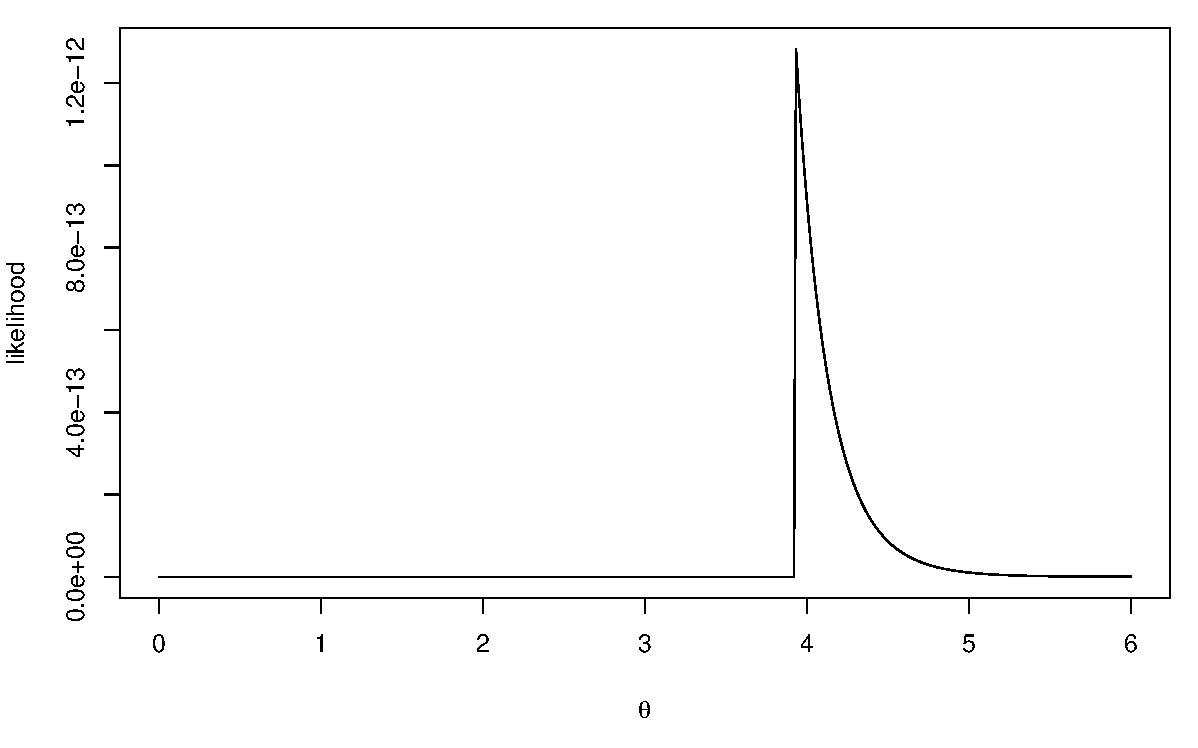
\includegraphics[width=6cm]{plots/likeliuniform.pdf}\vspace*{-1cm}
\end{center}
\begin{itemize}
    \item $L(\theta )$ is not differentiable at $\max_{i}x_{i}$
    \item Maximum is at $\hat{\theta}=\max_{i}x_{i}$
    \item The estimator is consistent but not asymptotically normal
    \item Illustration in R
\end{itemize}
\end{frame}


\begin{frame}\frametitle{Maximum likelihood}\framesubtitle{Dependent observations}
\begin{itemize}
    \item Maximum likelihood estimation is still possible if the observations are dependent
    \item The joint density of the observations
    \begin{equation*}
        f_{X_{1},\ldots ,X_{T}}\left( x_{1},\ldots ,x_{T}\right)
    \end{equation*}
    can be factorized as
    \begin{equation*}
    f_{X_{1}}(x_{1})\cdot \prod_{t=2}^{T}f_{X_{t}|X_{1}=x_{1},\ldots,X_{t-1}=x_{t-1}}\left( x_{t}\right)
    \end{equation*}
\end{itemize}
\end{frame}


\begin{frame}\frametitle{Maximum likelihood}\framesubtitle{Dependent observations}
\begin{itemize}
    \item Loglikelihood
    \begin{equation*}
        \ln L=\ln f_{X_{1}}(x_{1})+\sum_{t=2}^{T}\ln f_{X_{t}|X_{1}=x_{1},\ldots,X_{t-1}=x_{t-1}}\left( x_{t}\right)
    \end{equation*}
    \item If $T$ is large, one may ignore $\ln f_{X_{1}}(x_{1})$
    \item Computing the loglikelihood is straightforward if
    \begin{equation*}
        f_{X_{t}|X_{1}=x_{1},\ldots ,X_{t-1}=x_{t-1}}\left( x_{t}\right)=f_{X_{t}|X_{t-1}=x_{t-1}}\left( x_{t}\right)
    \end{equation*}
\end{itemize}
\end{frame}


\end{document}
